\section{Auswertung}
\label{sec:Auswertung}

\subsection{Wheatstonsche Brückenschaltung}
Für $R_2$ wurde ein Widerstand mit $R_2=\qty{332(9,96)}{\ohm}$ verwendet.
Der Fehler der Bauteile wird im Folgenden immer als $\pm\qty{3}{\percent}$ angenommen.
Der zu bestimmende Widerstand war Wert 13.
Durch das varieren der Widerstände $R_3$ und $R_4$, bis die Brückenspannung den Wert 0 annimmmt, wurden für diese bei der ersten Messung die Werte
$R_3=\qty{490}{\ohm}$ und $R_4=\qty{510}{\ohm}$ bestimmt, mit dem Verhältnis $\frac{R_3}{R_4}=0,961\pm0,005$.
Für den Fehler des Verhältnisses wurde $\pm\qty{0,5}{\percent}$ angenommen.
Mit Gleichung \ref{eqn:widerstand} ergibt sich $R_{13}=\qty{318,98}{\ohm}$.
Der Fehler dieser Größe wird mit Formel \ref{eqn:fehlerfortpflanzung} berechnet.
Damit ergibt sich hier $\increment R_{13}=\sqrt{ \Bigl(\frac{R_3}{R_4}\Bigr)^2 (\increment R_2)^2+(R_2)^2 \Bigl(\increment \frac{R_3}{R_4}\Bigr)^2}$.
Demnach gilt $R_{13}=\qty{318,98(9,71)}{\ohm}$.
Dies wurde für einen Weiteren unbekannten Widerstand, Wert 11, durchgeführt.
Hier ergibt sich $R_3=\qty{596}{\ohm}$, $R_4r=\qty{404}{\ohm}$ und $\frac{R_3}{R_4}=1,475\pm0,007$.
Daraus folgt mit Formel \ref{eqn:widerstand} und \ref{eqn:fehlerfortpflanzung} $R_{11}=\qty{490(15)}{\ohm}$.

\subsection{Kapazitive Brückenschaltung}
Für $R_2$ wird hier der selbe Wert wie bei der Wheatstonschen Brücke genutzt und die Kapizität des Kondensators $C_2$ ist $C_2=\qty{750(22,5)}{\nano\farad}$.
Die unbekannte Kapazität war hier Wert 8.
Durch das varieren von $R_3$ und $R_4$ bis ein Minumum gefunden wurde, wurden die Werte $R_3=\qty{675}{\ohm}$ und $R_4=\qty{325}{\ohm}$ aufgenommen.
Das Verhältnis der Werte beträgt $\frac{R_3}{R_4}=2,08\pm0,01$. 
Mit Gleichung \ref{eqn:widerstand} und \ref{eqn:fehlerfortpflanzung} ergibt sich $R_8=\qty{690(21)}{\ohm}$.
Die Kapazität $C_8$ kann mit Gleichung \ref{eqn:kapazität} und der Fehler mit Gleichung \ref{eqn:fehlerfortpflanzung} berechnet werden.
Der Fehler ist also $\increment C_{8}=\sqrt{ \Bigl(\frac{R_4}{R_3}\Bigr)^2 (\increment C_2)^2+(-C_2 \frac{R_4^2}{R_3^2})^2 \Bigl(\increment \frac{R_3}{R_4}\Bigr)^2}$.
Damit gilt $C_8=\qty{361(11)}{\farad}$.\\

Dies wird analog mit Wert 9 durchgeführt.
Damit ist $R_3=\qty{595}{\ohm}$ und $R_4=\qty{405}{\ohm}$.
Einsetzen in Formel \ref{eqn:widerstand} und \ref{eqn:fehlerfortpflanzung} ergibt $R_9=\qty{488(15)}{\ohm}$.
Die Kapazität hat nach Einsetzen in Formel \ref{eqn:kapazität} und \ref{eqn:fehlerfortpflanzung} den Wert $C_9=\qty{511(7)}{\ohm}$.


Siehe \autoref{fig:plot} und \autoref{tab:tabelle}!
\subsection{Klirrfaktor}

\begin{table}
    \centering
    \caption{Brückenspannung in Abhängigkeit von der Frequenz}
    \label{frequenzen}
    \begin{tblr}{
        colspec={S S},
        row{1}={guard, mode=math},
    }
    \toprule
    f[Hz] & U_\text{Br}[mV] \\
    \midrule
    50    &  230    \\
    100   &  100    \\
    150   &  15     \\
    200   &  50     \\
    250   &  100    \\
    300   &  130    \\
    350   &  160    \\
    400   &  200    \\
    450   &  200    \\
    500   &  220    \\
    1000  &  280    \\
    1500  &  300    \\
    2000  &  300    \\
    2500  &  300    \\
    3000  &  310    \\
    3500  &  310    \\
    4000  &  310    \\
    4500  &  310    \\
    5000  &  310    \\
    \bottomrule
    \end{tblr}
\end{table}

Für die Eingangsspannung gilt hier $U_s=\qty{1}{V}$, die Kapazität der Kondensatoren beträgt jeweils $\qty{994}{\nano\farad}
\text{ und } \qty{992}{\nano\farad}$ und wird hier auf $\qty{993}{\nano\farad}$ gemittelt, da eigentlich gelten müsse, dass 
diese gleich sind, dies aber nicht realisierbar war. Desweiteren betrtägt $R'=\qty{332}{\ohm} \text{ und } R=\qty{1}{\kilo\ohm}$.
Die Bezeichnungen dieser Größen finden sich in \ref{fig:Wien} wieder.\\
Zur bestimmung des Klirrfaktors wird hier nur die zweite Oberwelle betrachtet. In Gleichung \ref{}, zu dessen Berechnung, vereinfacht
sich die Summe dann zu zu einem $U_2^2$. Also vereinfacht sich die Berechnung des Faktors zu 
\begin{equation}
    k=\frac{U_2}{U_1}
\end{equation}
, wobei $U_1$ hier die Eingangsspannung $U_s$ ist. $U_2$ wird dann mithilfe von Gleichung \ref{} berechnet, wobei $j=\Omega=2$ ist.
Damit lässt sich der Klirrfaktor berechnen als
\begin{equation}
    k=3 \frac{U_\text{Br}}{U_1} \sqrt{\frac{(1-\Omega^2)^2+9\Omega^2}{(\Omega^2-1)^2}}
    \label{eqn:klirr2}
\end{equation}
mit $\Omega=2$. Die einzusetzende Brückenspannung wird dann über den Vergleich zwischen $ f $ und $f_0$ bestimmt, wobei $f_0$
die Frequenz ist, die die Brückenspannung insgesamt minimiert. Durch die Anwendung von \ref{} zeigt sich, dass 
\begin{equation}
    f=2f_0
\end{equation}
für die zweite Oberwelle gelten muss. 

\begin{figure}
    \centering
    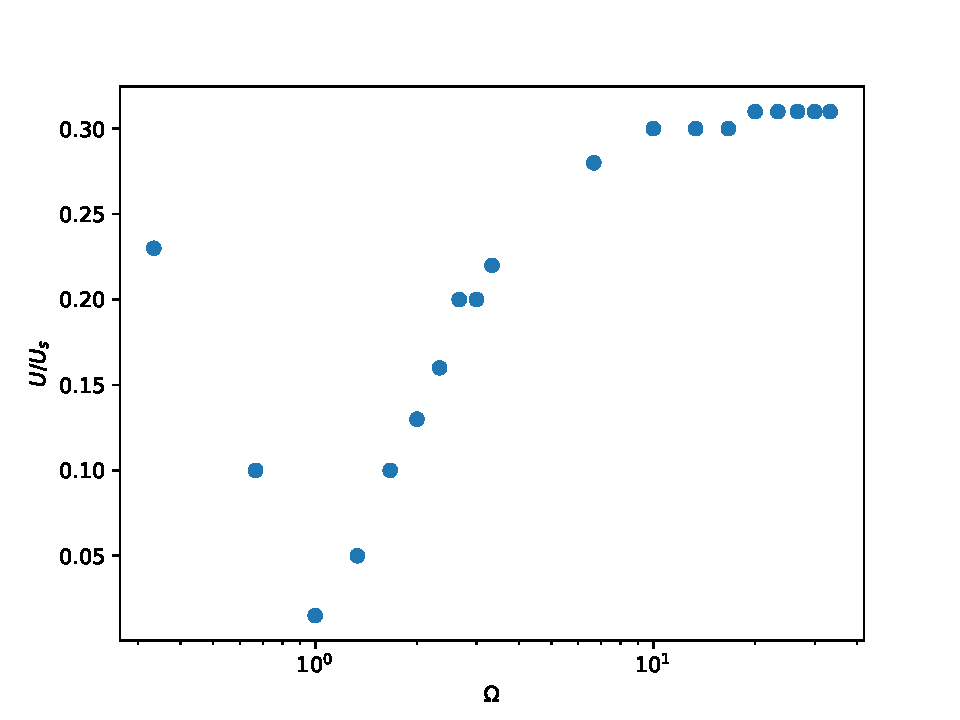
\includegraphics{ ./frequenzplot.pdf}
    \caption{Brückenspannung gegen Frequenzen}
    \label{fig:frequenzverhältnis}
\end{figure}

Aus \ref{frequenzen} ist abzulesen, dass $f_0=\qty{150}{\hertz}$ ist, woraus folgt,
dass die Brückenspannung, wenn $\Omega=2$ gilt, bei $f=\qty{300}{\hertz}$ abgelesen werden muss. Somit wird für k mit
$U_\text{Br}=\qty{130}{\milli\volt}$ gerechnet. Eingesetzt in \ref{eqn:klirr2} ist dann $k=0.87$.